\subsection{Throwing Using Sparse Reachable Map}\label{sec:sec:srm}

A Sparse Reachable Map (SRM) is used to create a collision free trajectories while having the end-effector reach a desired velocity as discribed in Lofaro et. al.\cite{dlofaro-srm}.
The SRM has been shown to be a viable method for trajectory generation for high degree of freedom, high-gain position controlled robots.  This remains true when operating without full knowledge of the reachable area as long as a good collision model of the robot is available. 
The end-effector velocity (magnitude and direction) is specified as well as a duration of this velocity. 
The SRM is created by making a sparse map of reachable end-effector positions in free space and the corresponding poses in joint space is created using random sampling in joint space and forward kinematics. 
The desired trajectory in free space is placed within the sparse map with the first point of the trajectory being a known pose from the original sparse map. 

\begin{equation}
L_d(0) \in SRM
\end{equation}

$L_d(0)$ is known both in joint space and in free space.
The Jacobian Transpose Controller method of inverse kinematics as described by Wolovich et al.\cite{4048118} is then used to find the subsequent points in the trajectory. 

\begin{equation}
q_1 = q_0 + \dot{q}_0 = q_0 + kJ^Te|_{x_0}^{x_1}
\end{equation}

Where $q_0$ and $x_0$ is the current pose and corresponding end-effector position respectively.  $q_1$ is the next pose for the next desired end-effector position $x_1$.
Each desired end-effector position $x$ must be within a euclidean distance $d$ (user defined) from any point in the SRM.

\begin{equation}
min \left(|x - SRM| \right) < d
\end{equation}

If one of the points in $x$ fails this criteria a new random point is chosen for $L_d(0)$ and the process is repeated.

Each pose in the trajectory is checked against the collision model to guarantee no self-collisions.  The collision model is based on the OpenRAVE model of the Hubo platform called OpenHUBO, see Fig~\ref{fig:vHubo}.

\begin{figure}[h]
  \centering
%\includegraphics[width=0.5\columnwidth]{./pictures/hubo1s.png}\includegraphics[width=0.5\columnwidth]{./pictures/hubo2s.png}
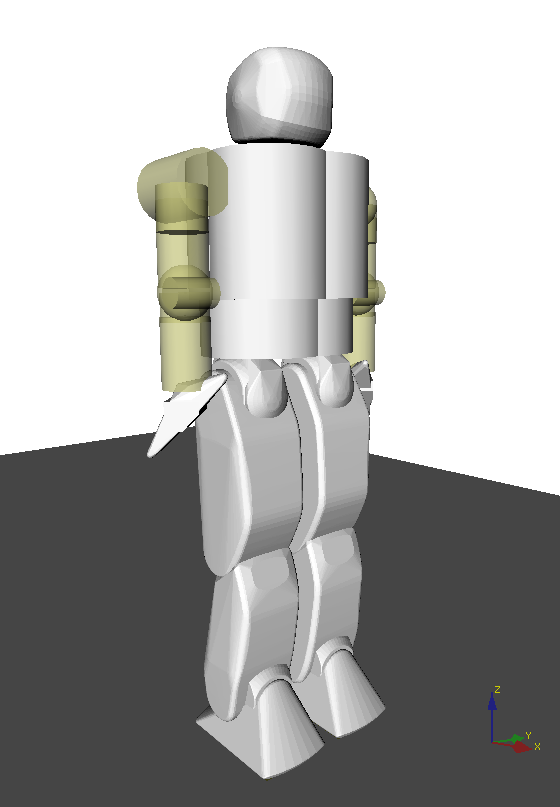
\includegraphics[width=0.5\columnwidth]{./pix/hCol.png}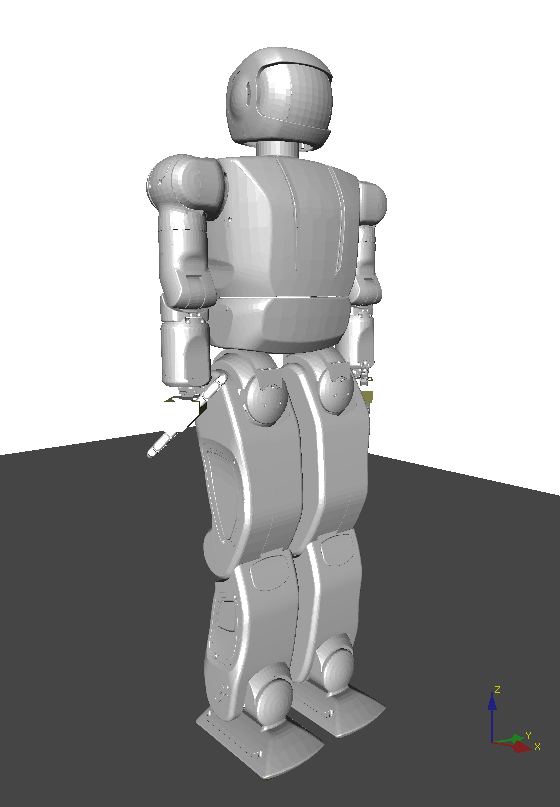
\includegraphics[width=0.5\columnwidth]{./pix/hBody.png}
  \caption{OpenHUBO - OpenRAVE model of Hubo KHR-4.  Left: Collision Geometry.  Right: Model with protective shells\cite{dlofaro-srm}.  }
  \label{fig:vHubo}
\end{figure}

The commanded trajectory produces the desired velocity of 4.9m/s at 60$^o$.  This was then tested on the OpenHUBO and on the Jaemi Hubo platform, Fig~\ref{fig:fThrow} and Fig~\ref{fig:3dThrowReal} respectively.



\begin{figure}[h]
  \centering
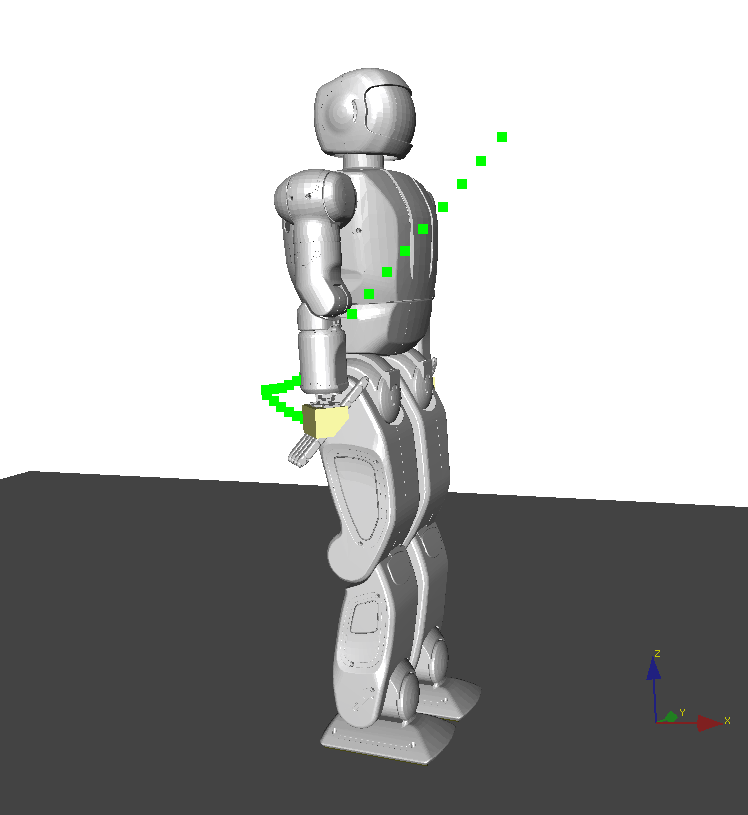
\includegraphics[width=0.25\columnwidth]{./pix/ddFinal/vHside1.png}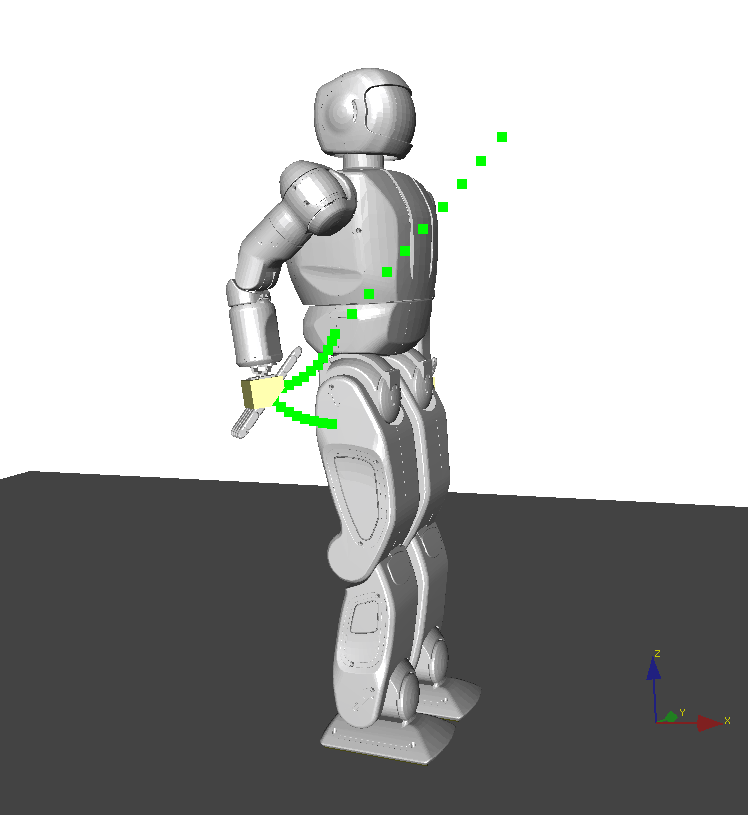
\includegraphics[width=0.25\columnwidth]{./pix/ddFinal/vHside3.png}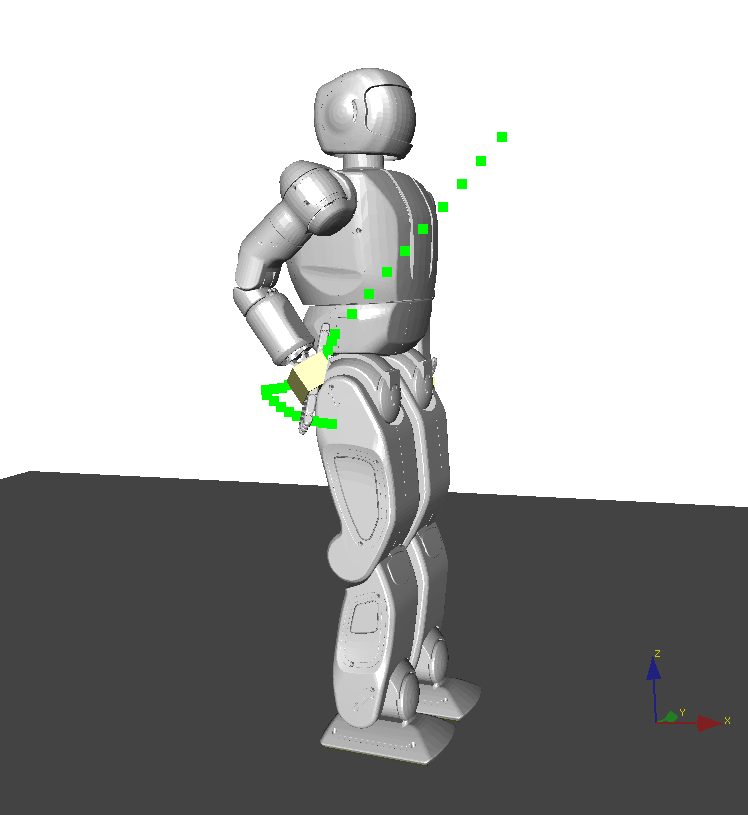
\includegraphics[width=0.25\columnwidth]{./pix/ddFinal/vHside4.png}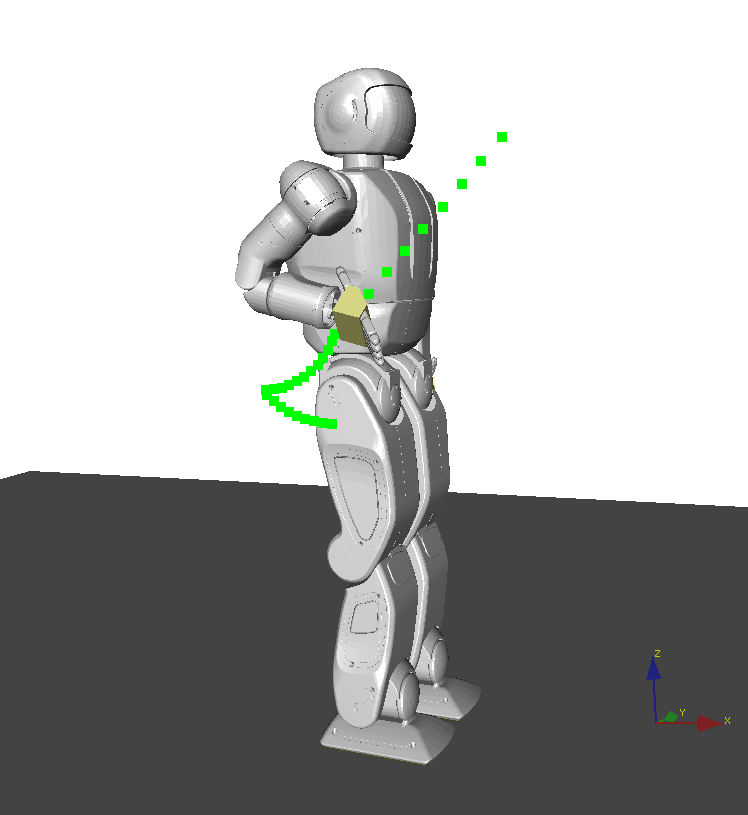
\includegraphics[width=0.25\columnwidth]{./pix/ddFinal/vHside5.png}
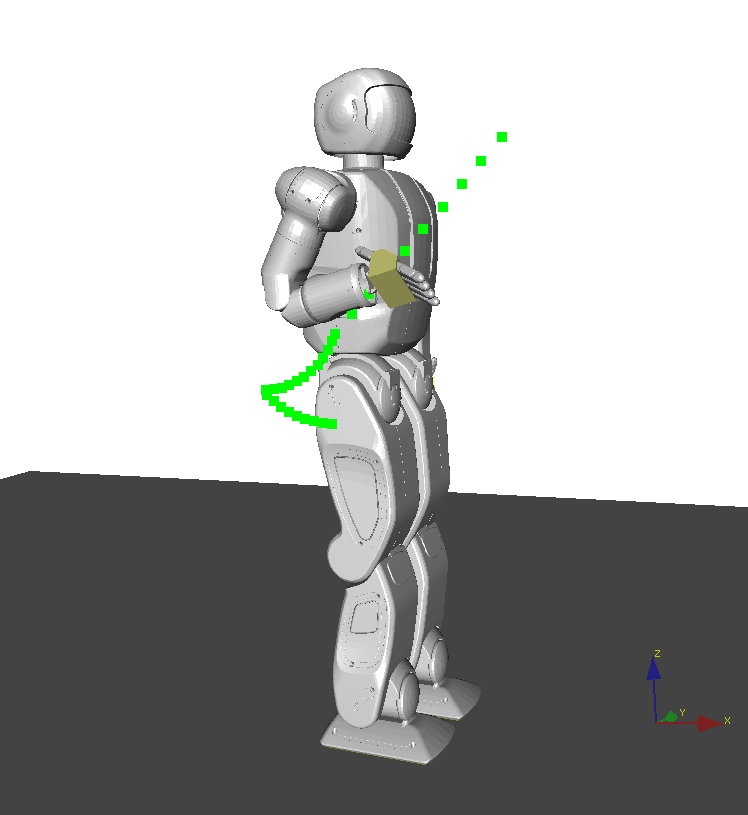
\includegraphics[width=0.25\columnwidth]{./pix/ddFinal/vHside6.png}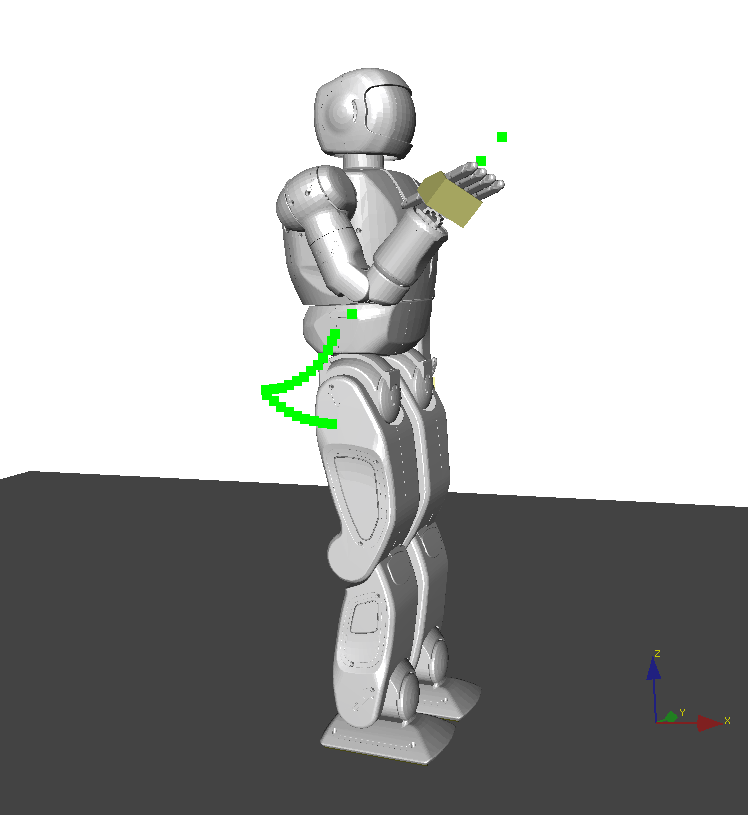
\includegraphics[width=0.25\columnwidth]{./pix/ddFinal/vHside7.png}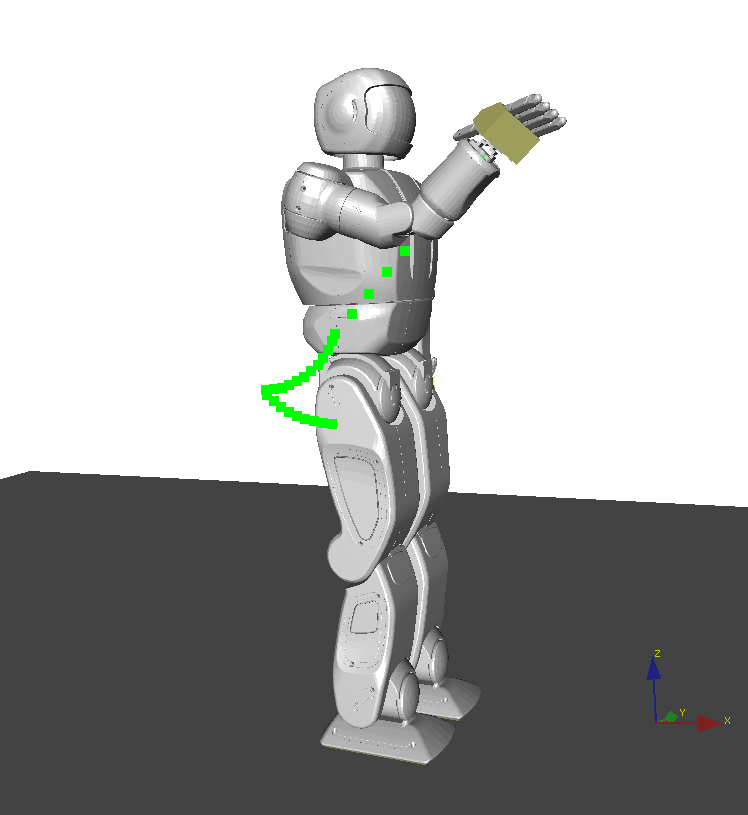
\includegraphics[width=0.25\columnwidth]{./pix/ddFinal/vHside9.png}
  \caption{OpenHUBO running the throwing trajectory immediately after the setup phase is completed.  $x_0$ is top left.  Frames are read left to right and have a $\Delta t$ of 0.15s\cite{dlofaro-srm}}
  \label{fig:fThrow}
\end{figure}

\begin{figure}[h]
  \centering
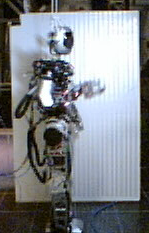
\includegraphics[width=0.25\columnwidth]{./pix/slowMotion/1.png}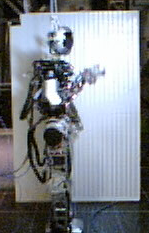
\includegraphics[width=0.25\columnwidth]{./pix/slowMotion/2.png}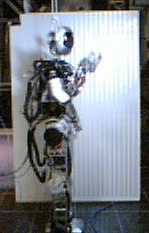
\includegraphics[width=0.25\columnwidth]{./pix/slowMotion/3.png}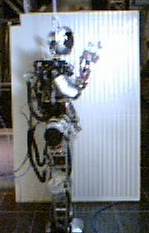
\includegraphics[width=0.25\columnwidth]{./pix/slowMotion/4.png}
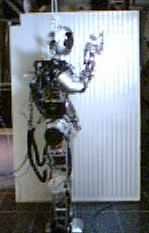
\includegraphics[width=0.25\columnwidth]{./pix/slowMotion/5.png}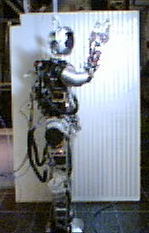
\includegraphics[width=0.25\columnwidth]{./pix/slowMotion/6.png}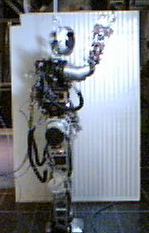
\includegraphics[width=0.25\columnwidth]{./pix/slowMotion/7.png}
  \caption{Jaemi Hubo running the throwing trajectory immediately after the setup phase is completed.  $x_0$ is top left.  Frames are read left to right and have a $\Delta t$ of 0.15s\cite{dlofaro-srm}}
  \label{fig:3dThrowReal}
\end{figure}

This method worked as desired however in approximately 10\% of the tests a joint would over torque and shutdown.  This is due to the system not taking the robots power limitations into account. 

